%!Mode:: "TeX:UTF-8"
%!TEX TS-program = xelatex
\documentclass{ctexart}
\usepackage{float}
\usepackage{tikz}
\usepackage{subfig}
\usetikzlibrary{patterns}
\newif\ifpreface
\prefacetrue
\usepackage{fontspec}
\usepackage{bbm}
\usepackage{tikz}
\usepackage{amsmath,amssymb,amsthm,color,mathrsfs}
\usepackage{fixdif}
\usepackage{hyperref}
\usepackage{cleveref}
\usepackage{enumitem}%
\usepackage{expl3}
\usepackage{lipsum}
\usepackage[margin=0pt]{geometry}
\usepackage{listings}
\definecolor{mGreen}{rgb}{0,0.6,0}
\definecolor{mGray}{rgb}{0.5,0.5,0.5}
\definecolor{mPurple}{rgb}{0.58,0,0.82}
\definecolor{backgroundColour}{rgb}{0.95,0.95,0.92}

\lstdefinestyle{CStyle}{
  backgroundcolor=\color{backgroundColour},
  commentstyle=\color{mGreen},
  keywordstyle=\color{magenta},
  numberstyle=\tiny\color{mGray},
  stringstyle=\color{mPurple},
  basicstyle=\footnotesize,
  breakatwhitespace=false,
  breaklines=true,
  captionpos=b,
  keepspaces=true,
  numbers=left,
  numbersep=5pt,
  showspaces=false,
  showstringspaces=false,
  showtabs=false,
  tabsize=2,
  language=C
}
\usetikzlibrary{calc}
\theoremstyle{remark}
\newtheorem{lemma}{Lemma}
\usepackage{fontawesome5}
\usepackage{xcolor}
\newcounter{problem}
\newcommand{\Problem}{\begin{tikzpicture}[baseline]%
    \node at (-0.02em,0.3em) {$\mathbb{P}$};%
    \node[scale=0.7] at (0.2em,-0.0em) {R};%
    \node[scale=0.7] at (0.6em,0.4em) {O};%
    \node[scale=0.8] at (1.05em,0.25em) {B};%
    \node at (1.55em,0.3em) {L};%
    \node[scale=0.7] at (1.75em,0.45em) {E};%
    \node at (2.35em,0.3em) {M};%
  \end{tikzpicture}%
}
\renewcommand{\theproblem}{\Roman{problem}}
\newenvironment{problem}{\refstepcounter{problem}\noindent\color{blue}\Problem\theproblem}{}

\crefname{problem}{\protect\Problem}{Problem}
\newcommand\Solution{\begin{tikzpicture}[baseline]%
    \node at (-0.04em,0.3em) {$\mathbb{S}$};%
    \node[scale=0.7] at (0.35em,0.4em) {O};%
    \node at (0.7em,0.3em) {\textit{L}};%
    \node[scale=0.7] at (0.95em,0.4em) {U};%
    \node[scale=1.1] at (1.19em,0.32em){T};%
    \node[scale=0.85] at (1.4em,0.24em){I};%
    \node at (1.9em,0.32em){$\mathcal{O}$};%
    \node[scale=0.75] at (2.3em,0.21em){\texttt{N}};%
  \end{tikzpicture}}
\newenvironment{solution}{\begin{proof}[\Solution]}{\end{proof}}
\title{\input{../../.subject}\input{../.number}}
\makeatletter
\newcommand\email[1]{\def\@email{#1}\def\@refemail{mailto:#1}}
\newcommand\schoolid[1]{\def\@schoolid{#1}}
\ifpreface
  \def\@maketitle{
  \raggedright
  {\Huge \bfseries \sffamily \@title }\\[1cm]
  {\Huge  \bfseries \sffamily\heiti\@author}\\[1cm]
  {\Huge \@schoolid}\\[1cm]
  {\Huge\href\@refemail\@email}\\[0.5cm]
  \Huge\@date\\[1cm]}
\else
  \def\@maketitle{
    \raggedright
    \begin{center}
      {\Huge \bfseries \sffamily \@title }\\[4ex]
      {\Large  \@author}\\[4ex]
      {\large \@schoolid}\\[4ex]
      {\href\@refemail\@email}\\[4ex]
      \@date\\[8ex]
    \end{center}}
\fi
\makeatother
\ifpreface
  \usepackage[placement=bottom,scale=1,opacity=1]{background}
\fi

\author{白永乐}
\schoolid{202011150087}
\email{202011150087@mail.bnu.edu.cn}

\def\to{\rightarrow}
\newcommand{\xor}{\vee}
\newcommand{\bor}{\bigvee}
\newcommand{\band}{\bigwedge}
\newcommand{\xand}{\wedge}
\newcommand{\minus}{\mathbin{\backslash}}
\newcommand{\mi}[1]{\mathscr{P}(#1)}
\newcommand{\card}{\mathrm{card}}
\newcommand{\oto}{\leftrightarrow}
\newcommand{\hin}{\hat{\in}}
\newcommand{\gl}{\mathrm{GL}}
\newcommand{\im}{\mathrm{Im}}
\newcommand{\re }{\mathrm{Re }}
\newcommand{\rank}{\mathrm{rank}}
\newcommand{\tra}{\mathop{\mathrm{tr}}}
\renewcommand{\char}{\mathop{\mathrm{char}}}
\DeclareMathOperator{\ot}{ordertype}
\DeclareMathOperator{\dom}{dom}
\DeclareMathOperator{\ran}{ran}

\begin{document}
\large
\setlength{\baselineskip}{1.2em}
\ifpreface
  \backgroundsetup{contents={%
    \begin{tikzpicture}
      \fill [white] (current page.north west) rectangle ($(current page.north east)!.3!(current page.south east)$) coordinate (a);
      \fill [bgc] (current page.south west) rectangle (a);
\end{tikzpicture}}}
\definecolor{word}{rgb}{1,1,0}
\definecolor{bgc}{rgb}{1,0.95,0}
\setlength{\parindent}{0pt}
\thispagestyle{empty}
\begin{tikzpicture}%
  % \node[xscale=2,yscale=4] at (0cm,0cm) {\sffamily\bfseries \color{word} under};%
  \node[xscale=4.5,yscale=10] at (10cm,1cm) {\sffamily\bfseries \color{word} Graduate Homework};%
  \node[xscale=4.5,yscale=10] at (8cm,-2.5cm) {\sffamily\bfseries \color{word} In Mathematics};%
\end{tikzpicture}
\ \vspace{1cm}\\
\begin{minipage}{0.25\textwidth}
  \textcolor{bgc}{王胤雅是傻逼}
\end{minipage}
\begin{minipage}{0.75\textwidth}
  \maketitle
\end{minipage}
\vspace{4cm}\ \\
\begin{minipage}{0.2\textwidth}
  \
\end{minipage}
\begin{minipage}{0.8\textwidth}
  {\Huge
    \textinconsolatanf{}
  }General fire extinguisher
\end{minipage}
\newpage\backgroundsetup{contents={}}\setlength{\parindent}{2em}

\else
  \title{Logic 3}
  \maketitle
\fi
\newgeometry{left=2cm,right=2cm,top=2cm,bottom=2cm}
%from_here_to_type
\begin{problem}\label{pro:1}
  下列命题各属于何种性质的命题?其主项的周延情况如何?
  \begin{enumerate}
    \item 无论什么困难都不是不可克服的。
    \item 有些动物不是用鳃呼吸的。
  \end{enumerate}
\end{problem}
\begin{solution}
  \begin{enumerate}
    \item 全称否定命题。主项周延。
    \item 特称否定命题。主项不周延。
  \end{enumerate}
\end{solution}
\begin{problem}\label{pro:2}
  用欧拉图表示性质命题的主项(S)和谓项(P)的关系。
  \begin{enumerate}
    \item 已知``有\(S\)是\(P\)''为真,请用欧拉图表示\(S\)和\(P\)之间的各种关系,并举出实例。
    \item 已知``所有\(S\)都不是\(P\)''为假,请用欧拉图表示\(S\)和\(P\)之间的各种关系,并举出实例。
  \end{enumerate}
\end{problem}
\begin{solution}
  \begin{enumerate}
    \item
      \begin{itemize}
        \item
          \begin{figure}[H]
            \centering
            \begin{tikzpicture}
              \filldraw[fill=white] (-2,-2) rectangle (3,2);
              \draw (0,0) circle (1)
              (1,0) circle (1);
              \node at (-0.2,1.2) {S};
              \node at (1.2,1.2) {P};
              \node at (0.5,0) {\checkmark};
            \end{tikzpicture}
            \label{fig:2.1.1}
          \end{figure}
          令\(S\)为奇数,\(P\)为质数。
        \item
          \begin{figure}[H]
            \centering
            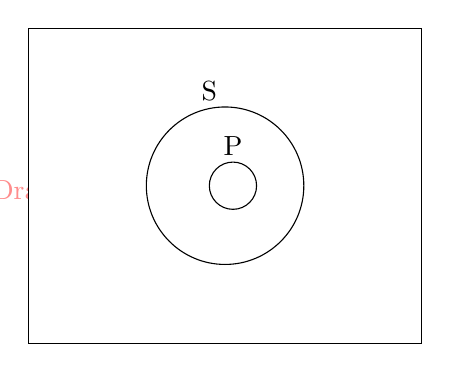
\begin{tikzpicture}
              \filldraw[fill=white] (-2,-2) rectangle (3,2);
              \draw (0.5,0) circle (1)
              (0.6,0) circle (0.3);
              \node at (0.3,1.2) {S};
              \node at (0.6,0.5) {P};
            \end{tikzpicture}
            \label{fig:2.1.2}
          \end{figure}
          令\(S\)为整数,\(P\)为偶数。
        \item
          \begin{figure}[H]
            \centering
            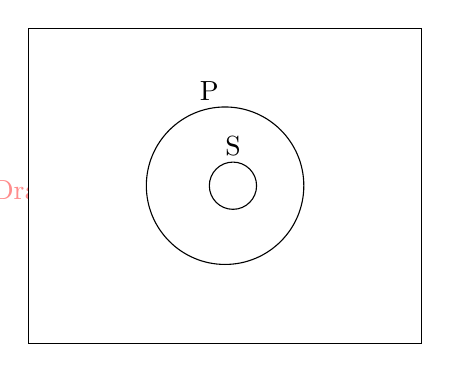
\begin{tikzpicture}
              \filldraw[fill=white] (-2,-2) rectangle (3,2);
              \draw (0.5,0) circle (1)
              (0.6,0) circle (0.3);
              \node at (0.3,1.2) {P};
              \node at (0.6,0.5) {S};
            \end{tikzpicture}
            \label{fig:2.1.3}
          \end{figure}
          令\(S\)为质数,\(P\)为整数。
      \end{itemize}
    \item ``所有\(S\)不是\(P\)''为假,即``有\(S\)为\(P\)''为真。故与上一问相同。
  \end{enumerate}
\end{solution}
\begin{problem}\label{pro:3}
  下列根据对当关系所进行的推理是否有效?为什么?
  \begin{enumerate}
    \item 有些人是画家,所以,有些人不是画家。
    \item 并非所有的办公大楼都是五层的,所以,有些办公大楼不是五层的。
  \end{enumerate}
\end{problem}
\begin{solution}
  \begin{enumerate}
    \item 无效。根据下反对关系,\(I\)假,\(O\)真假不定。
    \item 有效。根据矛盾关系,\(A\)假,\(O\)必真。
  \end{enumerate}
\end{solution}
\begin{problem}\label{pro:4}
  下列直接推理能否成立?如能成立,请用公式写出它的推理过程。
  \begin{enumerate}
    \item 从\(SAP\)真,推出\(\overline{P}O \overline{S}\)真。
    \item 从\(SEP\)真,推出\(\overline{P}I \overline{S}\)真。
  \end{enumerate}
\end{problem}
\end{document}
